% Work-MAT -- 2. rocnik, hodina 04. Grafy inverznich funkci.
\documentclass[11pt,a4paper]{article}
\input{../../sablony/pripravy/priprava.sty}
\usepackage{tikz}
\usetikzlibrary{arrows.meta}
\nastavPripravu{2. ročník}{Inverzní funkce}{04}{Inverzní funkce II: grafy}
\begin{document}
\poznamka{Hlavní myšlenka: graf inverze vznikne záměnou souřadnic, nikoli překlopením přes osu $x$ nebo $y$. Orientačně 5 min opakování, 12 min tabulka a graf, 10 min protipříklady, 12 min samostatná práce, 6 min kontrola a závěr. V případě potřeby využij milimetrový papír.}

\blok{Záměna vstupu a výstupu}
U prosté funkce platí: pokud $f(a)=b$, pak $f^{-1}(b)=a$. Bod $[a;b]$ grafu $f$ tak odpovídá bodu $[b;a]$ grafu $f^{-1}$. Geometricky jde o osovou souměrnost podle přímky $y=x$.

\begin{zadaniBox}[title={Věta - Souměrnost grafu inverzní funkce}]
Grafy funkce $f$ a její inverzní funkce $f^{-1}$ jsou osově souměrné podle přímky $y=x$.
\end{zadaniBox}
\noindent\textbf{Zdůvodnění.}\enspace Bod $[a;b]$ leží na grafu $f$ právě tehdy, když $b=f(a)$. Proto $a=f^{-1}(b)$ a bod $[b;a]$ leží na grafu $f^{-1}$. Záměna obou souřadnic je přesně zrcadlení podle $y=x$.


\begin{prikladReseniBox}[title={Příklad 1}]
Na $\mathbb R$ je dána $f(x)=2x+1$. Sestav tabulku tří bodů a tabulku odpovídajících bodů inverzní funkce. Urči její předpis.
\tcblower
\[
\begin{array}{c|rrr}
x&-1&0&1\\\hline f(x)&-1&1&3
\end{array}
\qquad
\begin{array}{c|rrr}
x&-1&1&3\\\hline f^{-1}(x)&-1&0&1
\end{array}
\]
Ze vztahu $y=2x+1$ dostaneme $x=(y-1)/2$. Tedy $f^{-1}(x)=(x-1)/2$.
\end{prikladReseniBox}

\begin{center}
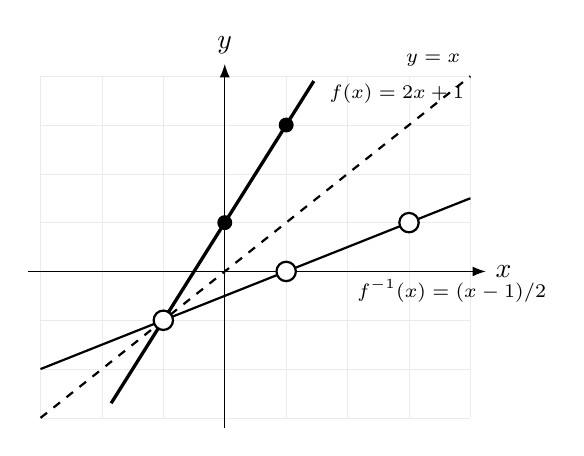
\begin{tikzpicture}[x=.78cm,y=.62cm,>=Latex]
\draw[step=1,gray!16,very thin](-3,-3)grid(4,4);
\draw[->](-3.2,0)--(4.25,0)node[right]{$x$};\draw[->](0,-3.2)--(0,4.25)node[above]{$y$};
\draw[dashed,thick](-3,-3)--(4,4)node[above left,font=\scriptsize]{$y=x$};
\draw[very thick,domain=-1.85:1.45]plot(\x,{2*\x+1});
\draw[thick,domain=-3:4]plot(\x,{(\x-1)/2});
\fill(-1,-1)circle(2.7pt) (0,1)circle(2.7pt) (1,3)circle(2.7pt);
\draw[fill=white,thick](-1,-1)circle(3.5pt) (1,0)circle(3.5pt) (3,1)circle(3.5pt);
\node[font=\scriptsize,anchor=west]at(1.55,3.65){$f(x)=2x+1$};
\node[font=\scriptsize,anchor=west]at(2,-.4){$f^{-1}(x)=(x-1)/2$};
\end{tikzpicture}
\end{center}
\poznamka{Černé plné body patří na graf původní funkce, bílé kružnice ukazují body inverze; společný bod $[-1;-1]$ leží na ose souměrnosti. Křivky jsou zobrazeny jen ve výřezu soustavy souřadnic.}

\blok{Inverze mění obor hodnot a definiční obor}
Jestliže $D(f)=\langle0;+\infty)$ a $H(f)=\langle1;+\infty)$, pak inverzní funkce musí mít $D(f^{-1})=\langle1;+\infty)$ a $H(f^{-1})=\langle0;+\infty)$; náčrtek to musí respektovat.

\begin{prikladReseniBox}[title={Příklad 2}]
U funkce $g(x)=x^2+1$ s $D(g)=\langle0;+\infty)$ rozhodni o prostotě a urči vzorec inverze a její definiční obor.
\tcblower
Funkce je na nezáporných argumentech rostoucí, a tedy prostá. Z $y=x^2+1$ s podmínkou $x\ge0$ plyne $x=\sqrt{y-1}$. Proto $g^{-1}(x)=\sqrt{x-1}$ a $D(g^{-1})=\langle1;+\infty)$.
\end{prikladReseniBox}

\poznamka{Názorně vysvětli, proč u příkladu 2 nebereme obě znaménka odmocniny: zadaná původní funkce přijímala jen $x\ge0$. Bez omezení oboru by inverze nebyla jednoznačná.}

\blok{Samostatná práce}
\begin{zadaniReseniBox}[title={Samostatná práce 1}]
\begin{enumerate}[label=\alph*)]
\item Pro body $A=[-2;1]$, $B=[0;3]$ a $C=[2;5]$ grafu prosté funkce napiš odpovídající body grafu inverze.
\item Urči inverzi k $f(x)=x-4$ na $\mathbb R$ a zakresli obě přímky v jedné soustavě.
\item Má $h(x)=x^2$ na $\mathbb R$ inverzní \emph{funkci}? Zdůvodni.
\end{enumerate}
\tcblower
\begin{enumerate}[label=\alph*)]
\item $A'=[1;-2]$, $B'=[3;0]$, $C'=[5;2]$.
\item $f^{-1}(x)=x+4$; grafy jsou souměrné podle $y=x$.
\item Nemá, protože není prostá: například pro výstup $4$ existují vstupy $-2$ i $2$.
\end{enumerate}
\end{zadaniReseniBox}

\begin{zadaniReseniBox}[title={Rozšíření 1}]
Průsečíky grafu funkce a její inverze mohou ležet mimo přímku $y=x$. Najdi příklad prosté funkce na $\mathbb R$, jejíž graf se s grafem inverze protíná i jinde.
\tcblower
Například $f(x)=-x$ je prostá a $f^{-1}(x)=-x$. Oba grafy splývají na celé přímce $y=-x$; mimo bod $[0;0]$ leží jejich společné body mimo $y=x$.
\end{zadaniReseniBox}

\begin{zadaniReseniBox}[title={Domácí úkol}]
\begin{enumerate}[label=\alph*)]
\item Vypočítej inverzní funkci k $f(x)=3x+6$ a zkontroluj $f^{-1}(f(2))$.
\item Jsou-li $[2;7]$ a $[-1;1]$ body grafu prosté funkce $g$, napiš dva odpovídající body grafu $g^{-1}$.
\end{enumerate}
\tcblower
\begin{enumerate}[label=\alph*)]
\item $f^{-1}(x)=(x-6)/3$ a $f^{-1}(f(2))=f^{-1}(12)=2$.
\item $[7;2]$ a $[1;-1]$.
\end{enumerate}
\end{zadaniReseniBox}
\end{document}
